\chapter{NILM As An Application} 
The last couple of years have the number of smart meters installed in residential houses increased drastically. The motivation for installing smart meters in the different houses have been to better understand energy consumption, in order to better plan energy distribution and production. Whit the smart meter came a golden opportunity for \ab{NILM}, since the equipment and infrastructure needed to measure the consumption and transfer the results to the internet was available in many households. 

The applications proposed in many of the articles published about \ab{NILM} focuses on energy management. Either it is for the electricity producers, that needs it to better predict consumption\fxnote{find ref}, or it is for the resident of the house that can optimize power usage to obtain savings. Even though these are fine examples of the potential usages of \ab{NILM} there might also exist a opportunity for the electric companies to sell the \ab{NILM} information and act as a data broker. This chapter contains a small case study to illustrate this point. 

\fxnote{Many of these claims need refs}

\section{The TV Rating Case}

\begin{figure}[H]
\centering
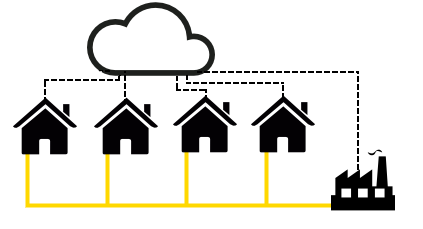
\includegraphics[width=0.7\textwidth]{billeder/CaseIlu.png}
\caption{Frequency comparison of the reconstruction methods}
\label{fig:SLC}
\end{figure}

\section{Results}


\section{Chapter Discussion}

